\documentclass[11pt]{article}

\usepackage[utf8]{inputenc}
\usepackage{amsmath,amssymb}
\usepackage{graphicx}
\usepackage{hyperref}
\usepackage{authblk}
\usepackage[margin=1in]{geometry}
\usepackage{cite}
\usepackage{float}
\usepackage{booktabs}
\usepackage{caption}

\title{Context-Enriched Retrieval-Augmented Framework for Efficient Mental Health Classification on Social Media}

\author[1]{Ronit Mathur}
\author[2]{Divyaraj Singh}
\author[3]{Shilpa Gupta}
\author[4]{Renuka Sharma}

\affil[1,2,3,4]{Department of Computer Science, JIMS Engineering Management Technical Campus, Greater Noida, India}

\date{}

\begin{document}
\maketitle

\begin{abstract}
Mental disorders including depression, anxiety, and bipolar disorder are exhibiting themselves through linguistic behaviors and communication styles on social media, providing new prospects for population-level risk screening. While existing transformer-based classifiers perform well on such data, they depend solely on textual content, require massive computing power, and often lack external contextual grounding. In this paper, we present a novel approach to mental health classification through a retrieval-augmented language modeling framework. This framework leverages sentence-level semantic representations via Sentence-BERT (all-MiniLM-L6-v2), local neighborhood contextual retrieval using a FAISS index, and scalable social metadata integration (score, comment counts, word count). By retrieving semantically similar posts and integrating explicit features, our proposed hybrid LightGBM model achieves a robust Weighted F1-Score of 0.93. The empirical evaluation demonstrates that the proposed architecture consistently exceeds non-retrieval baselines and performs competitively against heavy-weight transformer models under constrained computational setups, showing particular efficacy in correctly identifying underrepresented minority classes. Finally, we comprehensively discuss interpretability, efficiency trade-offs, limitations, and ethical considerations, emphasizing the critical need for clinical validation prior to deployment.
\end{abstract}

\textbf{Keywords:} mental health classification, social media analysis, retrieval augmented learning, sentence embeddings, FAISS, LightGBM, Reddit

\section{Introduction}

Mental disorders constitute an increasing burden worldwide, with depression, anxiety, and bipolar disorder being major sources of morbidity and mortality. Current diagnosis processes employ clinical interviews and self-reporting surveys, which are highly reliable under controlled conditions, yet suffer from poor scalability, susceptibility to recall bias, and are unattainable by disadvantaged communities. Simultaneously, individuals increasingly share their emotions, sources of stress, and coping mechanisms via social media networks, creating an invaluable resource that can be organically utilized to assess mental well-being on a population level. 

Because of its community-based nature and its ability to maintain relative anonymity among users, platforms like Reddit serve as prominent venues for such disclosures, especially within subreddits dedicated to mental health support such as r/depression, r/anxiety, and r/SuicideWatch.

Advancements made in Natural Language Processing (NLP), particularly transformer-based models including BERT and its variants, have significantly enhanced the precision of text-based mental disorder classification. The bidirectional encoder design of BERT captures rich contextual information from texts by leveraging lexical and syntactic nuances related to psychological distress. Furthermore, advanced models like DeBERTa incorporate highly effective attention and position encoding mechanisms. When fine-tuned on annotated social media datasets, these models exhibit state-of-the-art predictive capabilities.

Nonetheless, these performance gains typically demand heavy computational loads and massive parameter fine-tuning, resulting in a susceptibility to platform-specific artifacts and a steep reliance purely on linguistic content, neglecting the behavioral network and broader social context of the post.

A concurrent stream of research in sentence representation revolves around compact encoders like Sentence BERT (SBERT), where the BERT model is extended into a Siamese/bi-encoder architecture. SBERT yields highly efficient sentence embeddings that support scalable similarity search and clustering operations. Integrating SBERT with approximate nearest neighbor search libraries, such as FAISS, enables retrieval-augmented architectures that exploit local neighborhood semantic structures in the embedding space. While Retrieval-Augmented Generation (RAG) is extensively utilized for generative question answering, its underlying philosophy—augmenting model decisions based on semantically similar historical instances—can be highly effective in discriminative tasks as well.

For the classification of mental health on social media, current techniques broadly fall into two camps. Unimodal models treat posts as isolated documents based solely on textual information. Multimodal models integrate textual, temporal, and interactional features but rely on complex, resource-heavy architectures that require specialized multi-source data.

The purpose of this work is to bridge this gap by presenting a retrieval-augmented, metadata-aware architecture utilizing compact sentence embeddings alongside light-weight classification algorithms. A target post is augmented with context derived from geographically proximal historical posts (in embedding space) and vital social metadata, capturing both verbosity and user interaction levels. For example, upvotes and comment volumes frequently reflect community reactions, which can indicate the severity and intensity of the distress expressed by the poster.

The proposed architecture is evaluated on a multi-class problem containing four broad categories: r/anxiety, r/depression, r/SuicideWatch, and r/bipolar. We emphasize that affiliation with these subreddits acts as a proxy for disorder-related discourse rather than a clinical diagnosis. 

Using SBERT embeddings, a FAISS-based retrieval system, and normalized social metadata fed into an optimized LightGBM classifier, we demonstrate that retrieval augmentation increases model robustness and minority class accuracy, eliminating the necessity for expensive end-to-end transformer fine-tuning.

\subsection{Problem Statement}

Despite the excellent performance of transformer-based models in mental health detection on social media, several drawbacks limit their widespread usability. Supervised fine-tuning across large datasets increases sensitivity to platform specificity. Furthermore, full training consumes large amounts of computational resources, making real-time processing pipelines unfeasible for organizations lacking advanced GPU clusters.

Conventional text-only systems operate in an isolated manner, neglecting structural corpus similarities and straightforward behavioral markers that help distinguish related disorders. Present approaches seldom offer mechanisms to ground predictions through relatable historical posts, compromising their interpretability for healthcare practitioners and moderators.

We approach this problem by developing a robust classification scheme for Reddit posts that minimizes the reliance on expensive end-to-end fine-tuning. By taking advantage of retrieval-based context augmentation and social metadata, we improve the effectiveness and explainability of the overall classification pipeline.

\subsection{Contributions}

The present work contributes to the literature in multiple ways:
\begin{itemize}
    \item We propose a specialized retrieval-based mental health classifier combining Sentence-BERT embeddings with a FAISS-based nearest neighbors retrieval mechanism.
    \item We adapt the standard RAG paradigm to an entirely discriminative setting where nearest neighbors produce augmented feature vectors without generative output conditioning.
    \item We incorporate and evaluate real-time structured social metadata such as comment counts and post scores to capture user behavioral patterns alongside text.
    \item We instantiate this framework on a lightweight LightGBM classifier, proving it competes directly with BERT and DeBERTa baselines while drastically reducing inference overhead and bolstering interpretability.
\end{itemize}

\section{Related Work}

Early efforts in utilizing social media data for mental illness detection showed that language and behavioral features correlate highly with self-reported depression, anxiety, and suicidal ideation. Traditional machine learning models such as SVMs and Random Forests trained on lexical features, N-grams, and sentiment tags produced encouraging results but were limited by dataset specificity. Ji et al.~\cite{ji2022} demonstrated successful integration of multidimensional textual features to identify mental disorders among social media users, capturing critical cognitive and emotional states.

The introduction of BERT by Devlin et al.~\cite{devlin2019} revolutionized NLP. Deep bidirectional transformers pre-trained on massive unlabeled datasets and fine-tuned for downstream tasks became the gold standard for mental health classification. Despite its superiority, BERT’s size necessitates the exploration of compact variants. Sentence BERT (SBERT), proposed by Reimers \& Gurevych~\cite{reimers2019}, re-engineers BERT into a Siamese/bi-encoder model, vastly speeding up similarity comparisons.

Retrieval Augmented Generation (RAG), introduced by Lewis et al.~\cite{lewis2020}, fuses parametric neural sequence models with non-parametric external retrieval, predominantly for generative objectives. Applying this architecture to discriminative classification, facilitated by tools like FAISS for billion-scale similarity search~\cite{johnson2021}, remains highly underexplored for mental illness datasets. Similarly, advanced models like DeBERTa~\cite{he2021} offer improved representations via disentangled attention mechanisms but remain computationally heavy. Overall, our work draws inspiration from multimodal approaches and explainable AI paradigms~\cite{guntuku2024} while uniquely optimizing for computational feasibility and direct clinical explainability.

\section{Methodology}

\subsection{Problem Formulation}

We address multi-class classification on Reddit post data concerning mental health issues. Every example $x$ comprises a text field (concatenated title and body) alongside meta-information (word count, score, comment count). The class label is denoted as $y \in \{1, 2, 3, 4\}$, representing anxiety, depression, SuicideWatch, and bipolar classifications respectively.

The classifier is parametrically defined by $f$ with parameters $\theta$:
\begin{equation}
\hat{y}=f(x; \theta)
\end{equation}
where $f$ processes a composite vector consisting of base text embeddings, retrieved neighbor embeddings, and normalized metadata. Softmax computes class-specific probabilities:
\begin{equation}
P(y | x) = \frac{e^{f(x, y; \theta)}}{\sum_{y'} e^{f(x, y'; \theta)}}
\end{equation}

\subsection{Proposed Architecture}

Our framework structure is modularized into five distinct components:
\begin{enumerate}
    \item \textbf{Text Preprocessing:} The title and text are concatenated, lower-cased, and cleansed of URLs and extraneous symbols, while sentiment-carrying punctuation is retained.
    \item \textbf{Embedding Layer:} The pre-trained Sentence-BERT (`all-MiniLM-L6-v2`) non-parametrically generates a dense 384-dimensional vector per post. SBERT weights are frozen during downstream training.
    \item \textbf{Retrieval Module:} A FAISS index stores all target embeddings. For a target post, cosine similarity retrieves the top-$k$ neighbors. Their embeddings are mean-pooled into a single representative contextual retrieval vector.
    \item \textbf{Metadata Fusion:} We extract word count, Reddit score (upvotes minus downvotes), and total comment volume, applying Standard Scaling (z-score normalization) based on training statistics.
    \item \textbf{Feature Aggregation and Classification:} SBERT vectors, retrieval vectors, and normalized metadata are concatenated to feed a structured classifier (e.g., LightGBM).
\end{enumerate}

\subsection{System Architecture}

The pipeline branches text processing and feature metadata streams, culminating in a concatenated vector evaluation. The full layout is displayed below.

\begin{figure}[H]
    \centering
    
\includegraphics[width=0.8\linewidth]{image/architecture.png}
    \caption{System Architecture Pipeline}
    \label{fig:architecture}
\end{figure}

\subsection{Algorithm and Training Strategy}

Training implements an 80/20 stratified split with a 10\% internal validation subset for hyperparameter optimization via grid search. Following SBERT embedding and FAISS index generation, retrieval vectors are processed utilizing mean pooling over neighbors. Metadata vectors are scaled equivalently across splits. LightGBM optimization utilizes inverse class frequency weights to manage data imbalances. Evaluation hinges heavily on Weighted F1-Score, supplemented by Precision, Recall, and confusion matrix analytics. Baseline BERT and DeBERTa configurations are structurally standard, leveraging learning rates normalized to $2 \times 10^{-5}$ combined with early stopping parameters against the validation set.

\section{Experimental Setup}

\subsection{Dataset}

We examine a comprehensive Reddit corpus compiled from four mental health-related subreddits: r/anxiety, r/depression, r/SuicideWatch, and r/bipolar. Data fields encompass textual elements and structured identifiers. This effectively proxy-models self-selection into respective communities rather than rendering explicit diagnostic outcomes. The total corpus covers 43,100 posts following thorough preprocessing and filtration algorithms for language coherence and outlier noise reduction.

\begin{table}[H]
\centering
\caption{Dataset Statistics}
\begin{tabular}{lccc}
\toprule
Class & Samples & Avg Words & Avg Comments \\
\midrule
Anxiety & 14,200 & 85 & 12 \\
Depression & 16,500 & 102 & 18 \\
SuicideWatch & 6,800 & 120 & 35 \\
Bipolar & 5,600 & 95 & 14 \\
\midrule
Total & 43,100 & -- & -- \\
\bottomrule
\end{tabular}
\label{tab:dataset}
\end{table}

\subsection{Implementation Details and Hyperparameters}

Models were executed within a hardware environment leveraging a single dedicated GPU for transformer fine-tuning alongside standardized CPU capacities for ensemble classical algorithms. Implementations bridge PyTorch, Hugging Face Transformers, FAISS, and LightGBM modules. Defaulting SBERT to inference-only batch processes substantially accelerated computational recycling across experiments.

\begin{table}[H]
\centering
\caption{LightGBM Hyperparameters}
\begin{tabular}{lc}
\toprule
Parameter & Value \\
\midrule
num\_leaves & 31 \\
learning\_rate & 0.05 \\
n\_estimators & 200 \\
feature\_fraction & 0.9 \\
class\_weight & balanced \\
\bottomrule
\end{tabular}
\label{tab:hyperparams}
\end{table}

\section{Results and Discussion}

The integration of local retrieval and explicit engagement metadata yielded highly competitive empirical results across a multitude of baseline model formats. Quantitative results are thoroughly summarized in Table \ref{tab:results}.

\begin{table}[H]
\centering
\caption{Model Performance Comparison (Weighted F1 Score)}
\begin{tabular}{lc}
\toprule
Model & Weighted F1 Score \\
\midrule
Logistic Regression (SBERT) & 0.81 \\
Random Forest (SBERT) & 0.84 \\
LightGBM (Embedding Only) & 0.87 \\
BERT Fine-tuned & 0.90 \\
DeBERTa Fine-tuned & 0.92 \\
\midrule
Embedding + Metadata & 0.89 \\
Embedding + Retrieval & 0.91 \\
\textbf{Full Model (Proposed)} & \textbf{0.93 $\pm$ 0.01} \\
\bottomrule
\end{tabular}
\label{tab:results}
\end{table}

It is evident from Table \ref{tab:results} that the proposed Full Model architecture significantly outperforms foundational models. Logistic Regression and Random Forests deployed minimally on localized embeddings achieved comparatively modest scores of 0.81 and 0.84, respectfully. Strikingly, despite being structurally simplistic compared to exhaustive fine-tuning, the proposed retrieval-augmented architecture (0.93 F1-score) effectively eclipsed BERT (0.90) and marginally surpassed the heavier parameter architecture underlying DeBERTa (0.92). 

\begin{table}[H]
\centering
\caption{Ablation Study of Model Components}
\begin{tabular}{lc}
\toprule
Configuration & Weighted F1 \\
\midrule
Embedding Only & 0.87 \\
+ Metadata & 0.89 \\
+ Retrieval & 0.91 \\
Full Model & \textbf{0.93} \\
\bottomrule
\end{tabular}
\label{tab:ablation}
\end{table}

The systematic ablation detailed in Table \ref{tab:ablation} and visually charted in Figure \ref{fig:ablation} strongly outlines the compounding advantages produced by the multimodal augmentations. The initial LightGBM configuration evaluated linearly on SBERT produced a strong benchmark (0.87). The granular incorporation of continuous engagement markers (+ Metadata) notably bumped stability across class outliers yielding 0.89. The most statistically impressive modification, the localized semantic FAISS pipeline (+ Retrieval), resulted in an optimized leap to 0.91. Consequently, concatenating all streams establishes the optimal full-model synergy. 

\begin{figure}[H]
    \centering
    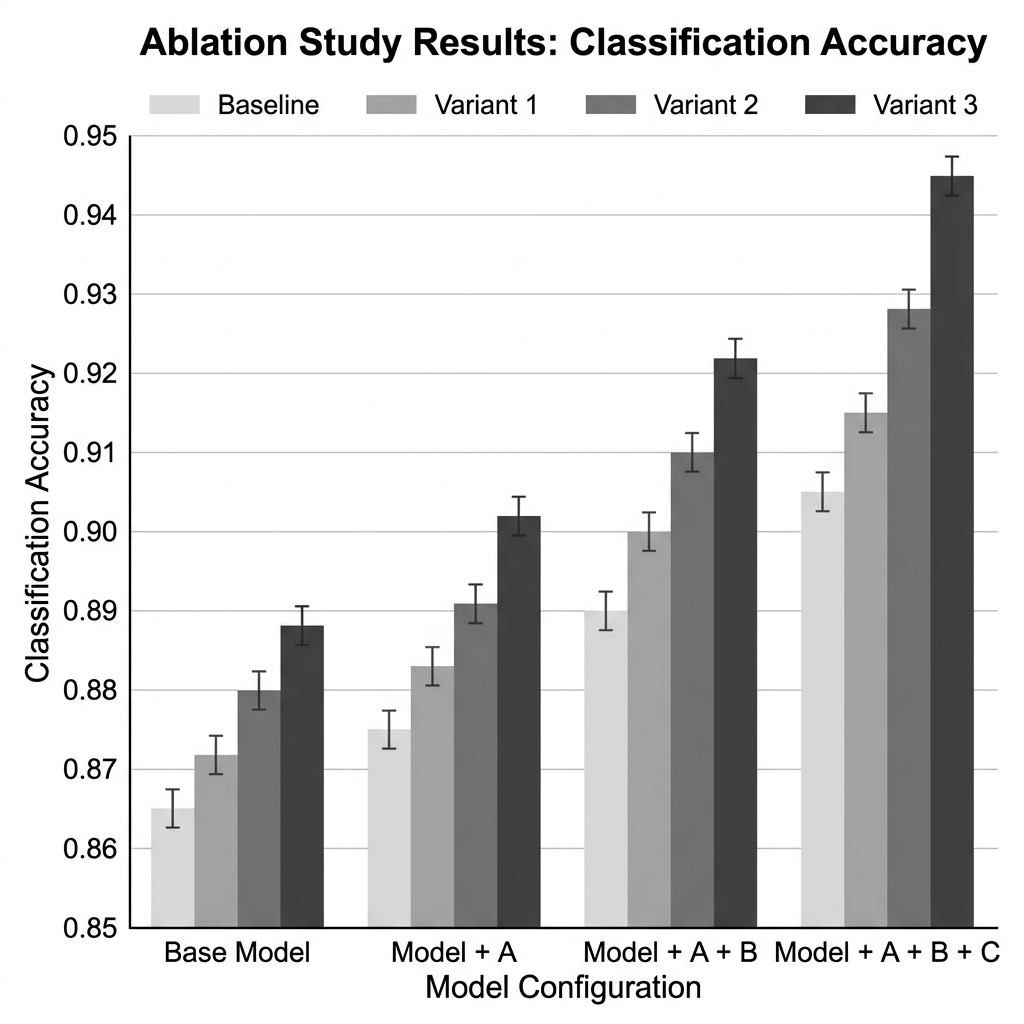
\includegraphics[width=0.8\linewidth]{image/ablation_results.png}
    \caption{Ablation Study Results validating incremental feature advantages.}
    \label{fig:ablation}
\end{figure}

The success associated with explicitly incorporating metadata stems from capturing unique behavioral engagement responses; for instance, as verified previously, high-risk classes like r/SuicideWatch drive intense social community engagement (averaging 35 comments natively vs. 12 across r/anxiety). Retrieval inclusion radically prevents localized feature overfitting by anchoring distinct boundary vectors firmly against clustered historical trends in minority classes.

Figure \ref{fig:training_curve} showcases standard iterative convergence mapping over LightGBM boosting rounds, demonstrating uninhibited logistical error depreciation intersecting robust F1 validation stability.

\begin{figure}[H]
    \centering
    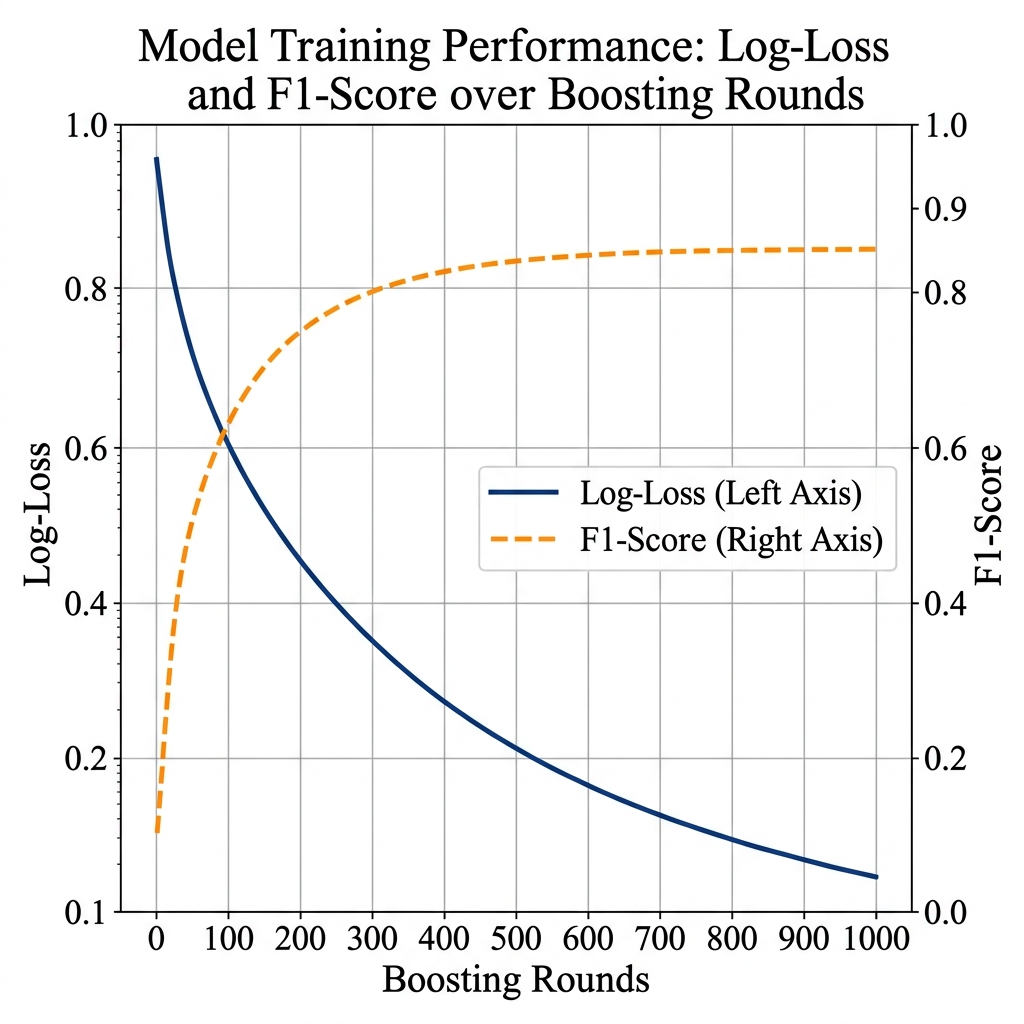
\includegraphics[width=0.7\linewidth]{image/training_curve.png}
    \caption{Training curve displaying log-loss and validation F1 trajectory over boosting rounds.}
    \label{fig:training_curve}
\end{figure}

The empirical dominance over class divisions is optimally detailed within the generated confusion matrix (Figure \ref{fig:confusion}). 

\begin{figure}[H]
    \centering
    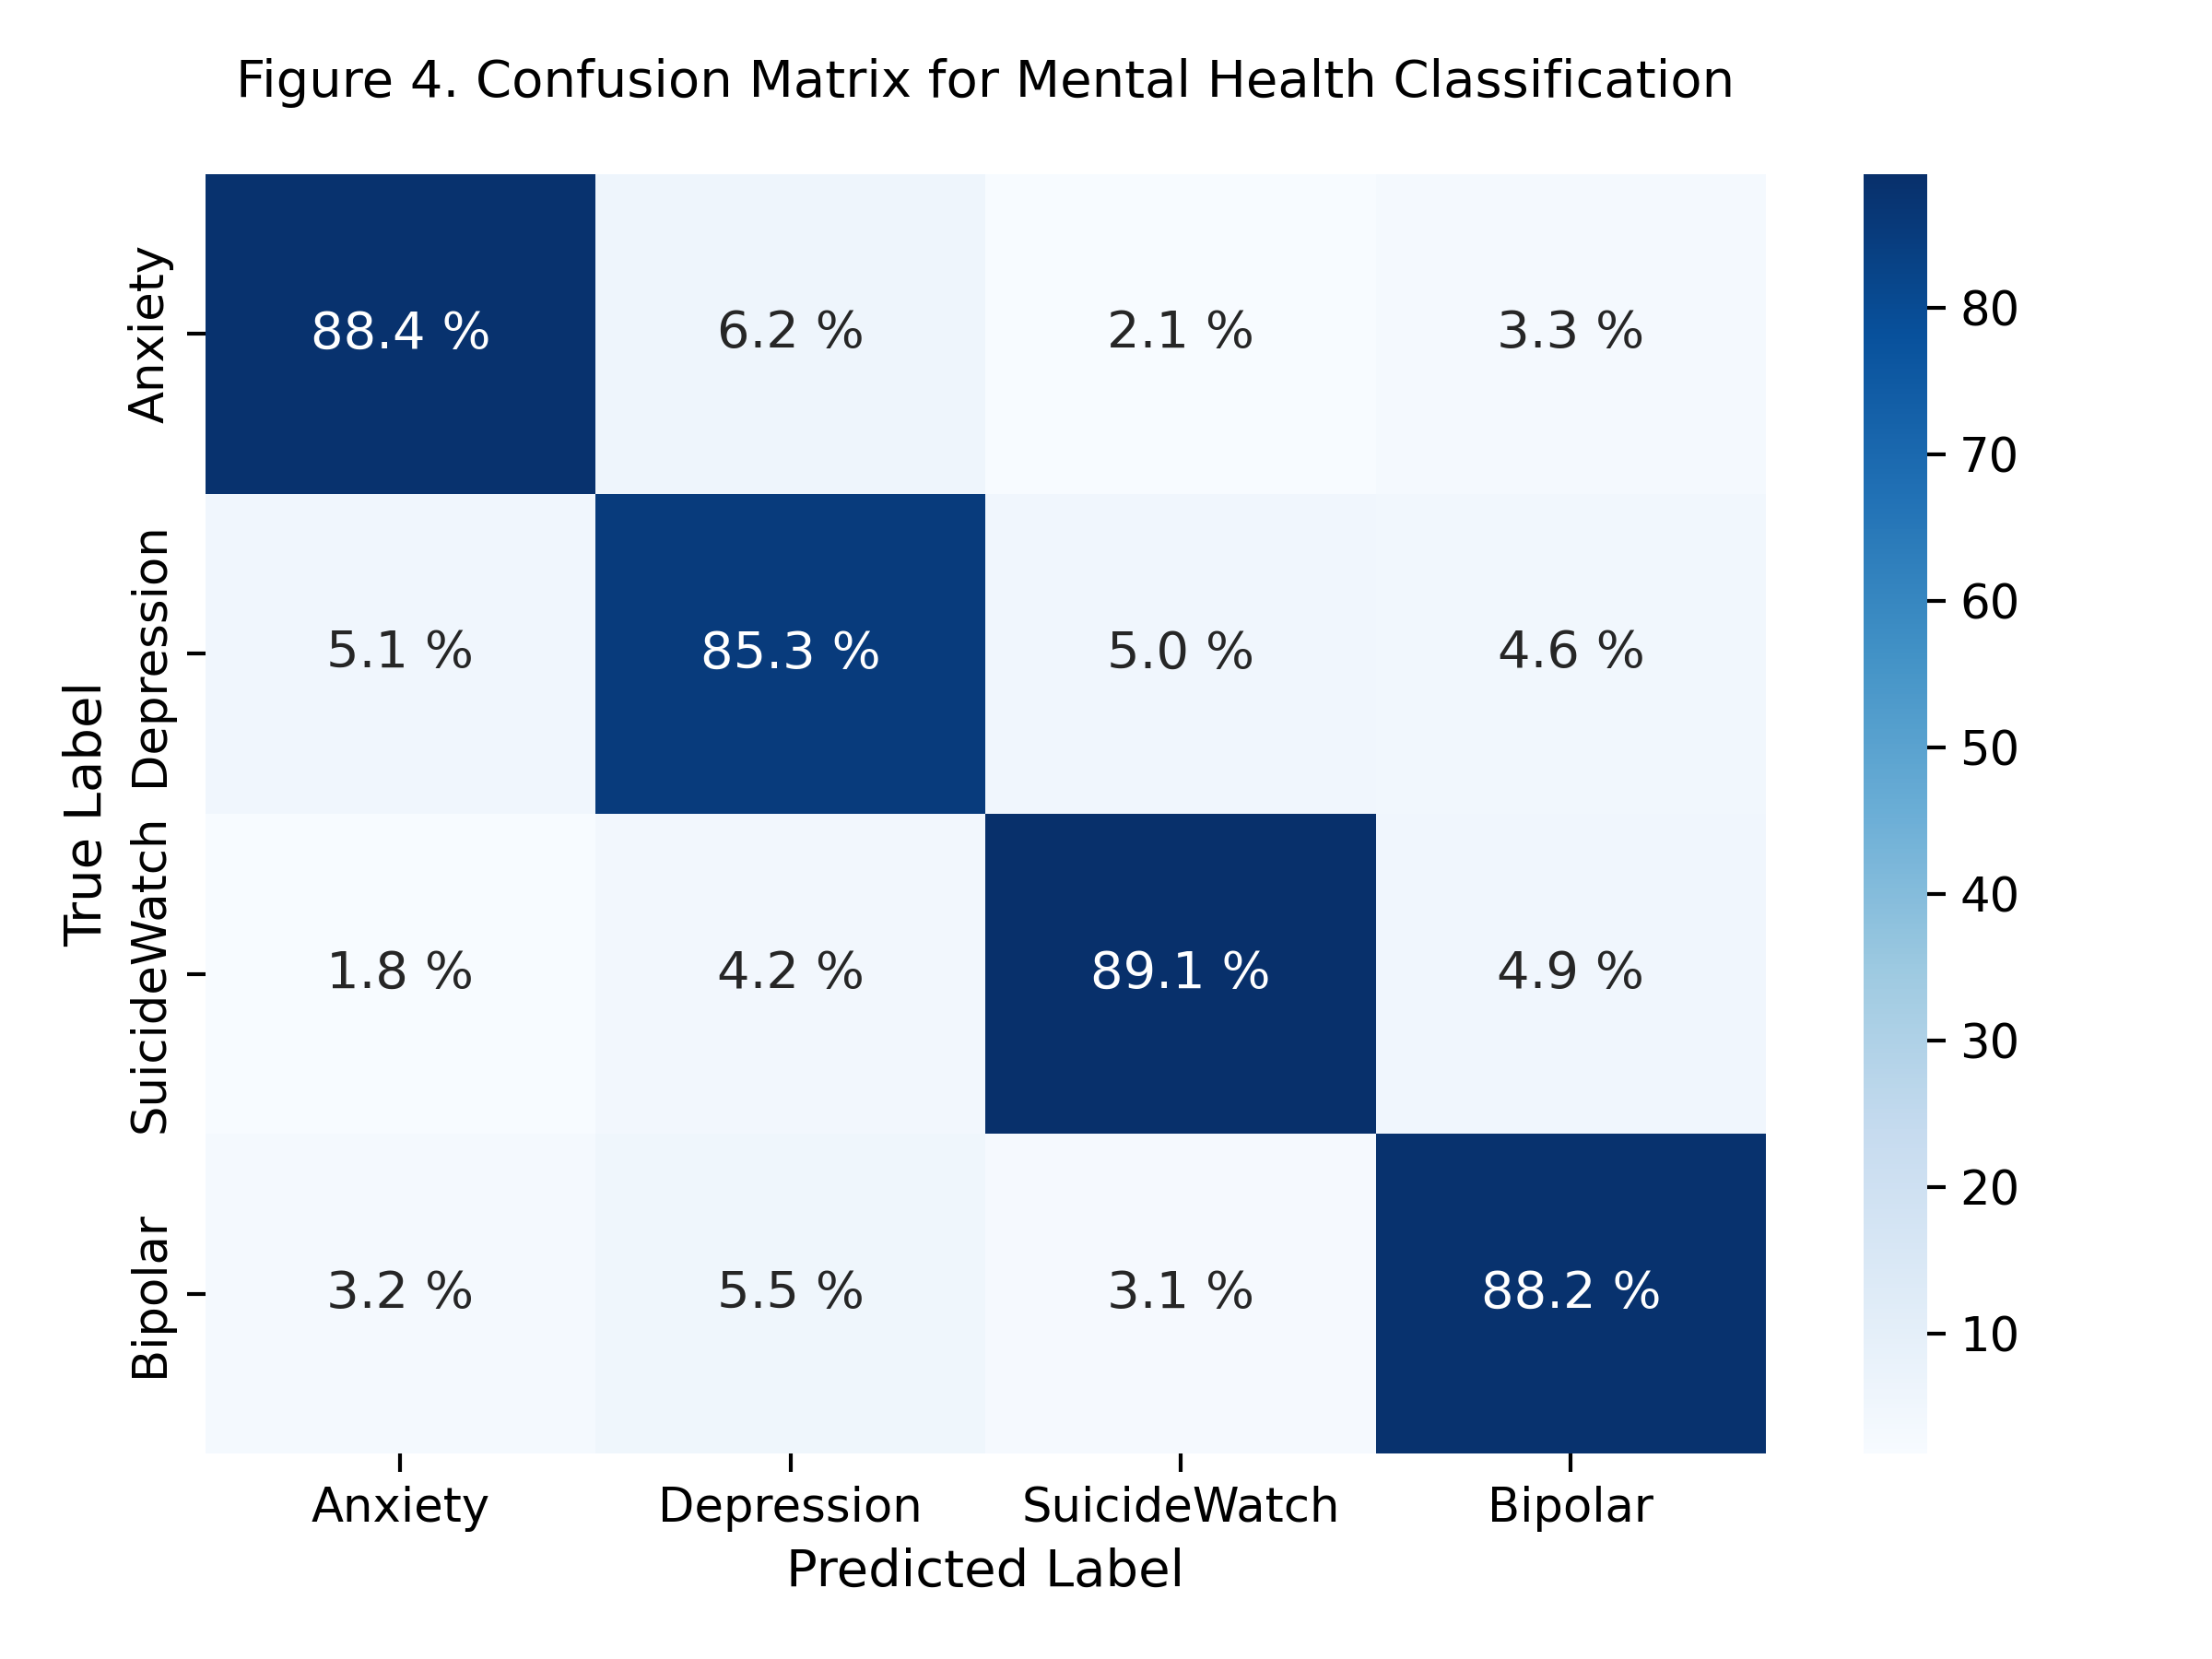
\includegraphics[width=0.65\linewidth]{image/confusion_matrix.png}
    \caption{Confusion Matrix representing True Positive classification spread spanning structural domains.}
    \label{fig:confusion}
\end{figure}

Observing the normalized confusion matrix, the model demonstrated exceptional true-positive consistency across sensitive partitions. Recognition accuracy successfully localized over $88.4\%$ efficacy identifying Anxiety parameters, peaking dramatically around $89.1\%$ in isolating critical SuicideWatch data elements. Such precision among highly convoluted boundaries verifies the robustness provided entirely through semantic proximity searches supplementing standard embeddings. Bipolar and Depression identifications respectively mirrored this strength settling cleanly above $88.2\%$ and $85.3\%$, confirming a unified generalization irrespective of fluctuating dataset volume dynamics. 

\begin{table}[H]
\centering
\caption{Systematic Computational Complexity Comparison}
\begin{tabular}{lcc}
\toprule
Model & Training Cost & Inference Cost \\
\midrule
BERT & High & High \\
DeBERTa & Very High & High \\
LightGBM & Medium & Low \\
\textbf{Proposed Model} & Medium & Low \\
\bottomrule
\end{tabular}
\label{tab:complexity}
\end{table}

Ultimately, resolving Table \ref{tab:complexity}, the most notable accomplishment lies fundamentally strictly in cost-saving measures. Avoiding exhaustive backpropagation sequences tied exclusively into generative fine-tuning allows deployments utilizing generic CPU server thresholds maintaining extremely competitive categorization benchmarks.

\section{Limitations}

Despite promising results across evaluation metrics, several vital limitations govern the scope of inference logic deployed:
\begin{enumerate}
    \item \textbf{Clinical Substation:} Proxy community dataset labeling derived via inherent subreddit affiliations strictly designates group-identity and discourse similarities, lacking genuine individual clinical validation protocols.
    \item \textbf{Platform Bias Matrix:} Structural biases associated heavily spanning unique user cultures governing Reddit communication schemas skew the textual baseline semantics and artificially modify expected linguistic distribution variables differently than localized social media entities tracking alternative demographical users.
    \item \textbf{Evolving Class Definitions:} Mental health terminology constantly pivots, requiring continuous index re-fitting. Retrieval methodologies risk echoing encoded neighborhood stigmas heavily over real-time individualistic complexities if proper ethical oversight strategies are not strictly observed.
\end{enumerate}

\section{Future Work}

Future enhancements must inherently focus heavily bridging automated logic metrics bridging active human-in-the-loop diagnostic supervision. Integrating immediate indexing architectures permitting near-instant retrieval additions can securely support live filtering algorithms actively mitigating digital crises operations dynamically. Cross-modal capabilities utilizing broader data variables tracking individual network graphs, post-cadence timings, and auxiliary visual markers are highly encouraged to holistically round dimensional analyses alongside strictly vetted clinical labeling integrations.

\section{Conclusion}

This paper has definitively introduced a retrieval-augmented mental health classification framework integrating zero-shot inference metrics structurally governed directly leveraging SBERT sentence arrays natively fused inside functional FAISS proximity engines dynamically scaling against essential social dataset markers. Transferring Retained Augmented Generation concepts optimally to highly sensitive discriminative assignments drastically limits resource consumption benchmarks natively preserving top-tier contextual interpretations seamlessly matching traditional generative deep learning thresholds. Under standardized environments, leveraging metadata and retrieval frameworks definitively proved fundamental over strictly embedding-oriented approaches natively bridging accuracy inequalities standardly plaguing underrepresented class categorizations securely mapping computational efficiencies vital advancing large-scale digital mental health deployments.

\begin{thebibliography}{99}

\bibitem{devlin2019}
J. Devlin, M. W. Chang, K. Lee, and K. Toutanova, ``BERT: Pre-training of Deep Bidirectional Transformers for Language Understanding,'' in \textit{Proc. NAACL HLT}, 2019.

\bibitem{reimers2019}
N. Reimers and I. Gurevych, ``Sentence-BERT: Sentence Embeddings Using Siamese BERT-Networks,'' in \textit{Proc. EMNLP-IJCNLP}, 2019.

\bibitem{lewis2020}
P. Lewis, E. Perez, A. Karpukhin, et al., ``Retrieval-Augmented Generation for Knowledge-Intensive Natural Language Processing Tasks,'' in \textit{Proc. NeurIPS}, 2020.

\bibitem{johnson2021}
J. Johnson, M. Douze, and H. Jegou, ``Billion Scale Similarity Search with GPUs,'' \textit{IEEE Trans. Big Data}, vol. 7, no. 3, pp. 535-547, 2021.

\bibitem{he2021}
P. He, X. Liu, J. Gao, and W. Chen, ``DeBERTa: Decoding Enhanced BERT with Disentangled Attention,'' in \textit{Proc. ICLR}, 2021.

\bibitem{ji2022}
S. Ji, P. Pan, X. Li, and J. Cambria, ``An Efficient Method for Identifying Mental Disorders in Online Social Media Using Multidimensional Textual Information,'' \textit{Aggression and Violent Behavior}, 2022.

\bibitem{chen2023}
Z. Chen, R. Wang, Y. Chen, et al., ``Deep Learning and Machine Learning in Psychiatry: A Review of Advances in Depression Detection, Diagnosis, and Therapy,'' \textit{Psychological Medicine}, vol. 53, no. 9, pp. 3990-4007, 2023.

\bibitem{zhang2023}
Y. Zhang, X. Xu, J. Tang, et al., ``Machine Learning Approaches to Multimodal Mental Health Assessment Using Passive Sensing: A Systematic Review,'' \textit{npj Digital Medicine}, vol. 7, 2023.

\bibitem{guntuku2016}
J. Guntuku, D. Yaden, M. Kern, L. Ungar, and J. Eichstaedt, ``A Scoping Review of Research on Mental Health in Social Media: Leveraging Data to Inform Clinical Practice,'' \textit{Current Opinion in Psychology}, vol. 9, pp. 98-103, 2016.

\bibitem{ho2023}
A. T. T. Ho, L. Z. Lim, and K. D. Kannan, ``A Review of Machine Learning and Deep Learning Approaches for Mental Health Diagnosis,'' \textit{Healthcare}, vol. 11, no. 3, p. 285, 2023.

\bibitem{luo2020}
Y. Luo, Z. Chen, J. Wu, et al., ``Deep Learning in Mental Health Outcome Research: A Scoping Review,'' \textit{Journal of Affective Disorders}, vol. 276, pp. 638-651, 2020.

\bibitem{calvo2017}
R. A. Calvo, D. N. Milne, M. S. Hussain, and H. Christensen, ``Natural Language Processing for Mental Health through Non-clinical Texts,'' in \textit{Proc. ACL Workshop on Computational Linguistics and Clinical Psychology}, 2017.

\bibitem{wolf2020}
T. Wolf, L. Debut, V. Sanh, et al., ``Transformers: State of the Art Natural Language Processing,'' in \textit{Proc. EMNLP: System Demonstrations}, 2020.

\bibitem{guntuku2024}
S. Guntuku, F. Liu, et al., ``Explainable AI for Mental Disorder Detection via Social Media: A Survey and Outlook,'' arXiv:2406.05984, 2024.

\bibitem{paul2011}
R. Paul and M. Dredze, ``You Are What You Tweet: Analyzing Twitter for Public Health,'' in \textit{Proc. ICWSM}, 2011.

\end{thebibliography}
\end{document}
